\documentclass[12pt,a4paper]{article}
\usepackage[utf8]{inputenc}
\usepackage[T1]{fontenc}
\usepackage{geometry}
\usepackage{graphicx}
\usepackage{amsmath}
\usepackage{amssymb}
\usepackage{booktabs}
\usepackage{array}
\usepackage{longtable}
\usepackage{multirow}
\usepackage{listings}
\usepackage{xcolor}
\usepackage{hyperref}
\usepackage{float}
\usepackage{caption}
\usepackage{subcaption}
\usepackage{tikz}
\usepackage{adjustbox}
\usetikzlibrary{shapes,arrows,positioning,fit,backgrounds}

\geometry{margin=1in}

\lstset{
    basicstyle=\ttfamily\footnotesize,
    breaklines=true,
    frame=single,
    numbers=left,
    numberstyle=\tiny,
    keywordstyle=\color{blue},
    commentstyle=\color{green!60!black},
    stringstyle=\color{red},
    language=Verilog,
    xleftmargin=2em,
    xrightmargin=1em
}

\title{\textbf{5-Stage Pipelined RISC-V CPU Core}\\
\large IC Design Laboratory Final Project Report}
\author{National Tsing Hua University\\IC Design Lab}
\date{Jan. 15, 2024}

\begin{document}

\maketitle

\begin{abstract}
This report presents a comprehensive design and implementation of a 5-stage pipelined RISC-V CPU core based on the RV32I instruction set architecture. The processor implements the classic five pipeline stages: Instruction Fetch (IF), Instruction Decode (ID), Execute (EX), Memory Access (MEM), and Write Back (WB). The design incorporates data hazard resolution through a forwarding unit and control hazard management via a stall unit. The processor was synthesized using Synopsys Design Compiler with the GPDK 45nm CMOS technology library, achieving a total area of 158,257.43 $\mu m^2$ and power consumption of 5.109 mW at 179.21 MHz operating frequency.
\end{abstract}

\tableofcontents
\newpage

%=============================================================================
\section{Introduction}
%=============================================================================

\subsection{Project Overview}

This project implements a 5-stage pipelined processor based on the RISC-V RV32I instruction set architecture. RISC-V is an open-source instruction set architecture (ISA) that has gained significant adoption in both academic and industrial applications due to its simplicity, modularity, and extensibility. The architecture follows the reduced instruction set computer (RISC) philosophy, emphasizing a small number of simple instructions that can be executed efficiently in a pipelined manner.

The design targets educational purposes while maintaining practical applicability, demonstrating fundamental concepts of computer architecture including pipelining, hazard detection, and data forwarding. By implementing the base integer instruction set (RV32I), the processor supports essential computational operations while keeping the design complexity manageable for verification and synthesis.

\subsection{Design Objectives}

The primary objective of this design is to create a fully functional 5-stage pipelined RISC-V processor that correctly executes the RV32I base integer instruction set. Beyond basic functionality, the design aims to implement efficient hazard detection and resolution mechanisms that maximize pipeline throughput while maintaining correctness. The forwarding unit enables most data hazards to be resolved without stalling, while the stall unit handles cases where forwarding alone is insufficient, such as load-use hazards.

Additionally, the design targets reasonable area and power consumption through synthesis optimization, making it suitable for implementation on FPGA platforms or ASIC fabrication. The verification methodology employs comprehensive simulation testing with randomly generated test patterns to ensure robust operation across diverse instruction sequences and hazard scenarios.

\subsection{Supported Instructions}

The processor supports the complete RV32I base integer instruction set, organized into several categories based on instruction format and functionality. Table~\ref{tab:instructions} summarizes the supported instructions.

\begin{table}[H]
\centering
\caption{Supported RISC-V Instructions}
\label{tab:instructions}
\footnotesize
\begin{tabular}{@{}lp{4.2cm}p{5.2cm}@{}}
\toprule
\textbf{Type} & \textbf{Instructions} & \textbf{Description} \\
\midrule
R-Type & ADD, SUB, XOR, OR, AND, SLL, SRL, SRA, SLT, SLTU & Register-register arithmetic and logical operations \\
\addlinespace
I-Type (ALU) & ADDI, XORI, ORI, ANDI, SLLI, SRLI, SRAI, SLTI, SLTIU & Immediate arithmetic and logical operations \\
\addlinespace
I-Type (Load) & LW, LB & Load word and load byte from memory \\
\addlinespace
S-Type & SW, SB & Store word and store byte to memory \\
\addlinespace
B-Type & BEQ, BNE & Conditional branch instructions \\
\addlinespace
J-Type & JAL & Jump and link \\
\addlinespace
I-Type (JALR) & JALR & Jump and link register \\
\addlinespace
U-Type & LUI, AUIPC & Load upper immediate, add upper immediate to PC \\
\bottomrule
\end{tabular}
\end{table}

R-type instructions perform register-to-register operations, taking two source operands from the register file and writing the result back to a destination register. I-type instructions use one register operand and one immediate value encoded in the instruction. Load instructions read data from memory, while store instructions write register values to memory. Branch instructions conditionally alter the program flow based on comparisons, and jump instructions provide unconditional control transfer with optional link register saving.

%=============================================================================
\section{Architecture Overview}
%=============================================================================

\subsection{Pipeline Structure}

The processor implements a classic 5-stage pipeline architecture, where each stage performs a specific function in the instruction execution process. This pipelined approach allows multiple instructions to be in various stages of execution simultaneously, significantly improving throughput compared to a single-cycle implementation.

\begin{figure}[H]
\centering
\begin{adjustbox}{max width=\textwidth}
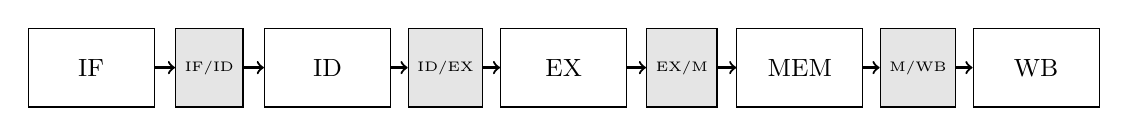
\begin{tikzpicture}[
    stage/.style={rectangle, draw, minimum width=1.6cm, minimum height=1cm, align=center, font=\small},
    reg/.style={rectangle, draw, fill=gray!20, minimum width=0.6cm, minimum height=1cm, font=\tiny},
    arrow/.style={->, thick}
]
    \node[stage] (IF) at (0,0) {IF};
    \node[reg] (IF_ID) at (1.5,0) {IF/ID};
    \node[stage] (ID) at (3,0) {ID};
    \node[reg] (ID_EX) at (4.5,0) {ID/EX};
    \node[stage] (EX) at (6,0) {EX};
    \node[reg] (EX_M) at (7.5,0) {EX/M};
    \node[stage] (MEM) at (9,0) {MEM};
    \node[reg] (M_RB) at (10.5,0) {M/WB};
    \node[stage] (WB) at (12,0) {WB};

    \draw[arrow] (IF) -- (IF_ID);
    \draw[arrow] (IF_ID) -- (ID);
    \draw[arrow] (ID) -- (ID_EX);
    \draw[arrow] (ID_EX) -- (EX);
    \draw[arrow] (EX) -- (EX_M);
    \draw[arrow] (EX_M) -- (MEM);
    \draw[arrow] (MEM) -- (M_RB);
    \draw[arrow] (M_RB) -- (WB);
\end{tikzpicture}
\end{adjustbox}
\caption{5-Stage Pipeline Structure with Pipeline Registers}
\label{fig:pipeline}
\end{figure}

The Instruction Fetch (IF) stage reads the next instruction from the instruction cache using the program counter value. The fetched instruction and program counter are then passed to the Instruction Decode (ID) stage through the IF/ID pipeline register. During the ID stage, the instruction is decoded to generate control signals, source register values are read from the register file, and immediate values are extracted and sign-extended.

The Execute (EX) stage performs arithmetic and logical operations using the ALU, computes memory addresses for load and store instructions, and evaluates branch conditions. Results from the EX stage flow into the Memory Access (MEM) stage, where load instructions read data from the data cache and store instructions write data to memory. Finally, the Write Back (WB) stage writes results back to the register file, completing the instruction execution.

\subsection{Module Hierarchy}

The top-level module \texttt{top\_riscv\_core} serves as the central integration point for all processor components. It instantiates the Program Counter (PC) module for managing instruction addresses, and the Instruction Cache (Icache) module implemented as a dual-port memory with two banks of 128 words each. The IF/ID pipeline register captures the fetched instruction and program counter values for the decode stage.

The decode stage components include the Register File (regfile) containing 32 general-purpose 32-bit registers, the Control Unit that generates all control signals based on the instruction opcode, and the Immediate Generator (imm\_gen) that extracts and sign-extends immediate values according to the instruction format. The Stall Unit detects hazard conditions requiring pipeline stalls, while the NOP Multiplexer inserts bubbles when stalls occur.

For the execute stage, the design includes the ID/EX pipeline register, the Forwarding Unit that detects and resolves data hazards, and the Arithmetic Logic Unit (ALU) that performs all computational operations. The EX/MEM pipeline register connects to the Data Cache (Dcache) module in the memory stage, which supports both word and byte access. The MEM/WB pipeline register completes the pipeline, feeding results back to the register file in the write-back stage.

%=============================================================================
\section{Detailed Module Descriptions}
%=============================================================================

\subsection{Program Counter (PC.v)}

The Program Counter module manages instruction address sequencing and handles various control flow scenarios including sequential execution, branches, and jumps. The module maintains a 32-bit program counter register that is updated on each clock cycle based on the selected next address source.

\begin{table}[H]
\centering
\caption{PC Module Interface Signals}
\label{tab:pc_interface}
\small
\begin{tabular}{@{}llcp{4.5cm}@{}}
\toprule
\textbf{Signal} & \textbf{Dir} & \textbf{Width} & \textbf{Description} \\
\midrule
clk & In & 1 & System clock \\
rst\_n & In & 1 & Active-low reset \\
boot\_up & In & 1 & Boot-up mode indicator \\
keep\_PC & In & 1 & Stall signal (hold PC) \\
branch\_valid & In & 1 & Branch/JAL taken signal \\
jalr\_M & In & 1 & JALR in MEM stage \\
alu\_result\_M & In & 32 & JALR target address \\
pc\_branch\_ID & In & 32 & Branch/JAL target address \\
pc & Out & 32 & Current PC value \\
pc\_running & Out & 1 & Indicates execution mode \\
\bottomrule
\end{tabular}
\end{table}

The PC module implements a three-state state machine (IDLE, LOAD, RUN) to manage the boot-up sequence and normal execution. During boot-up, the PC remains at zero while instructions are loaded into the instruction cache. Once boot-up completes, the module transitions to the RUN state and begins normal execution.

The next PC value is determined through priority-based selection. When \texttt{branch\_valid} is asserted (indicating a taken branch or JAL), the branch target from \texttt{pc\_branch\_ID} is selected. When \texttt{jalr\_M} is active, the ALU result from the MEM stage provides the JALR target address. When \texttt{keep\_PC} is asserted due to a stall condition, the current PC value is maintained. Otherwise, sequential execution proceeds with PC + 4.

\begin{lstlisting}[caption={PC Update Logic}]
assign pc_IF = pc + 4;
assign pc_running = (state == PC_RUN);

always@(posedge clk) begin
    if(~rst_n || (state != PC_RUN))
        pc <= 0;
    else
        pc <= pc_temp;
end

always@* begin
    case(1'b1)
        branch_valid: pc_temp = pc_branch_ID;
        jalr_M:       pc_temp = alu_result_M;
        keep_PC:      pc_temp = pc;
        default:      pc_temp = pc_IF;
    endcase
end
\end{lstlisting}

\subsection{Instruction Cache (Icache.v)}

The instruction cache is implemented as a dual-port memory structure to support both the boot-up sequence and normal instruction fetching operations. The memory is organized into two banks, \texttt{mem0} and \texttt{mem1}, with each bank containing 128 words of 32 bits. This provides a total capacity of 256 words or 1 KB of instruction storage. Bank selection is determined by address bit [7], allowing the full address space to be divided between the two banks.

During the boot-up phase when the write enable (\texttt{wen}) is asserted, the cache accepts instruction data through the boot interface. The boot address determines which bank receives the data, with addresses having bit [7] set going to \texttt{mem1} and others going to \texttt{mem0}. During normal operation, the cache provides the instruction at the address specified by the program counter. The dual-bank organization enables efficient access patterns and simplifies the boot loading process.

\begin{lstlisting}[caption={Icache Memory Read and Bank Selection}]
always@*
    rdata = (addr[7])? mem1[addr[6:0]]: mem0[addr[6:0]];
\end{lstlisting}

\subsection{Data Cache (Dcache.v)}

The data cache handles all load and store operations, supporting word-level and byte-level access. The memory is implemented as a single-port array of 128 words, each 32 bits wide, providing 512 bytes of data storage. Word accesses use bits [9:2] of the address for indexing (8 bits), though only the lower 7 bits effectively select among the 128 memory locations.

The access granularity is determined by the \texttt{funct3} field from the instruction: funct3=0 indicates byte access (LB/SB) and funct3=2 indicates word access (LW/SW). For byte loads, the least significant 8 bits are extracted from the memory word and sign-extended to 32 bits using bit [7]. Byte stores write only the lower 8 bits of the source register to the target memory location while preserving the upper 24 bits of the existing word.

\begin{lstlisting}[caption={Data Cache Access Logic}]
case(funct3)
    0: mem_n[i] = (MemWrite && (i == addr)) ?
                  {mem[i][31:8], rs2_rdata_M[7:0]} : mem[i];
    2: mem_n[i] = (MemWrite && (i == addr)) ?
                  rs2_rdata_M : mem[i];
    default: mem_n[i] = mem[i];
endcase
\end{lstlisting}

\subsection{Register File (regfile.v)}

The register file implements the 32 general-purpose registers specified by the RISC-V architecture. Each register is 32 bits wide, and the file provides two simultaneous read ports for source operands and one write port for the destination register. Register x0 is hardwired to zero, meaning any write to this register is ignored and reads always return zero.

The register file provides combinational read access, delivering the current register values on the same clock cycle as the address is presented. Register x0 is hardwired to zero by explicitly resetting it every cycle, ensuring that reads from x0 always return zero regardless of any write operations. Data hazards involving the register file are handled externally by the forwarding unit, which bypasses values from later pipeline stages when dependencies are detected.

\begin{lstlisting}[caption={Register File Implementation}]
assign rdata1 = gpr[raddr1];
assign rdata2 = gpr[raddr2];

always @(posedge clk) begin
    if (~srst_n) begin
        for(i = 0; i < 32; i = i + 1) gpr[i] <= 0;
    end
    else begin
        gpr[0] <= 0;  // x0 always zero
        for(i = 1; i < 32; i = i + 1)
            gpr[i] <= gpr_n[i];
    end
end

always @(*) begin
    for(i = 0; i < 32; i = i + 1)
        gpr_n[i] = (wen && (i == waddr)) ? wdata : gpr[i];
end
\end{lstlisting}

\subsection{Control Unit (Control.v)}

The control unit serves as the instruction decoder, generating all control signals needed to orchestrate the datapath based on the instruction opcode. The unit identifies instruction types by matching the 7-bit opcode field against known patterns for R-type, I-type, S-type, B-type, J-type, and U-type instructions.

\begin{table}[H]
\centering
\caption{Control Unit Output Signals}
\label{tab:control_signals}
\small
\begin{tabular}{@{}lcp{6cm}@{}}
\toprule
\textbf{Signal} & \textbf{Width} & \textbf{Description} \\
\midrule
ALU\_src & 1 & Selects ALU operand B (1=rs2, 0=imm) \\
ALU\_ctrl & 4 & Specifies ALU operation \\
branch & 1 & Indicates branch instruction \\
MemWrite & 1 & Enables memory write operation \\
jal & 1 & Indicates JAL instruction \\
jalr & 1 & Indicates JALR instruction \\
PMAItoReg & 2 & Write-back source (11=PC, 10=Mem, 01=ALU, 00=Imm) \\
rd\_wen & 1 & Enables register file write \\
\bottomrule
\end{tabular}
\end{table}

The control unit uses local parameters to define opcode values for each instruction type. R-type instructions use opcode 0110011 for register-register ALU operations, while I-type ALU instructions use 0010011. Load instructions are identified by opcode 0000011, and store instructions by 0100011. Branch instructions use opcode 1100011, JAL uses 1101111, and JALR uses 1100111. The U-type instructions LUI and AUIPC are identified by opcodes 0110111 and 0010111 respectively.

\subsection{Immediate Generator (imm\_gen.v)}

The immediate generator extracts immediate values from instructions and performs sign extension as required by each instruction format. RISC-V uses several different immediate encodings depending on the instruction type, and the generator handles all formats correctly.

For I-type instructions, the 12-bit immediate occupies instruction bits [31:20] and is sign-extended to 32 bits. S-type immediates are split between bits [31:25] and [11:7], requiring concatenation before sign extension. B-type branch offsets have an even more complex encoding with bits scattered across [31], [7], [30:25], and [11:8], plus an implicit zero in the least significant bit for halfword alignment. U-type immediates occupy the upper 20 bits [31:12] of the instruction and are placed in the upper 20 bits of the result. J-type jump offsets combine bits from [31], [19:12], [20], and [30:21] with an implicit zero for alignment.

\subsection{Arithmetic Logic Unit (ALU.v)}

The ALU performs all arithmetic and logical operations required by the instruction set. It accepts two 32-bit operands and a 4-bit control signal that specifies the operation to perform. The result is a 32-bit output value that is passed to subsequent pipeline stages.

\begin{table}[H]
\centering
\caption{ALU Operations and Control Codes}
\label{tab:alu_ops}
\small
\begin{tabular}{@{}cll@{}}
\toprule
\textbf{ALU\_ctrl} & \textbf{Operation} & \textbf{Description} \\
\midrule
4'b0000 & ADD & Addition of operands \\
4'b1000 & SUB & Subtraction (A - B) \\
4'b0001 & SLL & Shift left logical \\
4'b0010 & SLT & Set if less than (signed) \\
4'b0011 & SLTU & Set if less than (unsigned) \\
4'b0100 & XOR & Bitwise exclusive OR \\
4'b0101 & SRL & Shift right logical \\
4'b1101 & SRA & Shift right arithmetic \\
4'b0110 & OR & Bitwise inclusive OR \\
4'b0111 & AND & Bitwise AND \\
\bottomrule
\end{tabular}
\end{table}

The 4-bit ALU control code is formed by concatenating the funct7[5] bit with the 3-bit funct3 field: \texttt{ALU\_ctrl = \{funct7[5], funct3\}}. This encoding naturally distinguishes between operations that share the same funct3 value, such as ADD/SUB and SRL/SRA, which differ only in the funct7 bit.

The shift operations use only the lower 5 bits of the second operand as the shift amount, consistent with the RISC-V specification for 32-bit shifts. The SRA operation preserves the sign bit during right shifts, implementing arithmetic shifting for signed values. The comparison operations SLT and SLTU return 1 if the first operand is less than the second, and 0 otherwise, with SLT performing signed comparison and SLTU performing unsigned comparison.

%=============================================================================
\section{Pipeline Registers}
%=============================================================================

The design employs four pipeline registers to separate the five execution stages, enabling instructions at different stages to execute concurrently without interference. Each register captures the relevant signals at the rising clock edge and holds them stable for the subsequent stage to use.

The IF/ID register captures the fetched instruction along with the program counter and PC+4 values from the instruction fetch stage. These values are needed in the decode stage to extract instruction fields and compute branch and jump targets. The register also supports stall functionality, maintaining its current values when a stall condition is detected.

The ID/EX register holds significantly more information, including all control signals generated by the control unit, the register read data for both source operands, the sign-extended immediate value, register addresses for source and destination registers, and the function fields (funct3 and funct7) needed by the ALU control logic. This register bridges the decode and execute stages, ensuring all operands and control information are available for execution.

The EX/MEM register captures the ALU result, the data to be stored for store instructions, and control signals needed for the memory and write-back stages. For load instructions, this includes the computed memory address; for ALU instructions, it contains the result to be written back.

The MEM/WB register holds the memory read data for load instructions, the ALU result passed through from the execute stage, and write-back control signals. The write-back multiplexer uses these values to select the appropriate data for register file writes.

%=============================================================================
\section{Hazard Control}
%=============================================================================

\subsection{Data Hazards and Forwarding Unit}

Data hazards occur when an instruction depends on the result of a previous instruction that has not yet completed its write-back. Without proper handling, such dependencies would cause incorrect execution. The forwarding unit addresses this challenge by detecting dependencies and routing result values from later pipeline stages directly to where they are needed, bypassing the register file.

The design implements three forwarding multiplexers to handle different dependency scenarios. The \texttt{rs1\_ID\_fwd} multiplexer (3-bit) forwards data to the first source operand in the ID stage, while \texttt{rs2\_ID\_fwd} (3-bit) handles the second source operand. The \texttt{rs2\_EX\_fwd} multiplexer (2-bit) forwards data to the second operand in the EX stage, specifically for store instructions that need the store data.

The forwarding logic performs opcode-aware dependency checking, examining both the source and destination instruction types to determine when forwarding is valid. The forwarding unit considers register address matches, ensures the destination is not x0, and verifies that the instruction types support the forwarding path.

\begin{table}[H]
\centering
\caption{Forwarding Multiplexer Selection Values}
\label{tab:fwd_sel}
\small
\begin{tabular}{@{}clp{5.5cm}@{}}
\toprule
\textbf{Value} & \textbf{Source} & \textbf{Description} \\
\midrule
0 & Register file & No forwarding required \\
1 & EX stage ALU result & Forward from ID/EX stage \\
2 & MEM stage ALU result & Forward from EX/MEM stage \\
3 & MEM stage memory data & Forward load data from MEM \\
4 & WB stage write-back data & Forward from MEM/WB stage \\
5 & MEM stage PC value & Forward PC+4 for JAL linkage \\
\bottomrule
\end{tabular}
\end{table}

The forwarding multiplexers in the top module use these selection values to route the appropriate data to the operand inputs, bypassing the register file when data hazards are detected.

\subsection{Control Hazards and Stall Unit}

While forwarding resolves most data hazards, certain situations require pipeline stalls. The stall unit detects these conditions and generates a stall signal that freezes the PC and IF/ID register while inserting a bubble into the pipeline.

Load-use hazards occur when an instruction immediately following a load attempts to use the loaded value. Since the load data is not available until after the memory stage, forwarding cannot provide the value in time for the execute stage. The stall unit detects this by checking if the ID/EX stage contains a load instruction (MemRead active) and whether its destination register matches either source register of the instruction in the IF/ID stage.

Branch hazards arise when a branch instruction depends on a result not yet available. The design resolves branches in the ID stage for minimal penalty, but this requires the comparison operands to be ready. If a preceding instruction in the ID/EX stage will produce a needed operand, or if a load in the EX/MEM stage will provide a branch operand, the pipeline must stall until the data becomes available.

The stall unit generates three control signals: \texttt{keep\_PC} to freeze the program counter, \texttt{keep\_instr} to preserve the current instruction in the IF/ID register, and \texttt{nop\_sel} to insert a bubble via the NOP multiplexer.

\begin{lstlisting}[caption={Stall Detection Logic}]
always @(*) begin
    case(1'b1)
        // Load-use stall: load in EX, dependent in ID
        (opcode_EX == I_TYPE_LOAD && opcode_ID == R_TYPE):
            {keep_PC, keep_instr, nop_sel} =
                (rd_EX == rs1_ID || rd_EX == rs2_ID) ?
                3'b111 : 3'b000;
        // Load-branch stall: load in EX/MEM, branch in ID
        (opcode_EX == I_TYPE_LOAD && opcode_ID == B_TYPE):
            {keep_PC, keep_instr, nop_sel} =
                (rd_EX == rs1_ID || rd_EX == rs2_ID) ?
                3'b111 : 3'b000;
        (opcode_M == I_TYPE_LOAD && opcode_ID == B_TYPE):
            {keep_PC, keep_instr, nop_sel} =
                (rd_M == rs1_ID || rd_M == rs2_ID) ?
                3'b111 : 3'b000;
        // Branch resolution delay
        (opcode_EX == B_TYPE && ~(opcode_ID == J_TYPE)):
            {keep_PC, keep_instr, nop_sel} = 3'b111;
        default:
            {keep_PC, keep_instr, nop_sel} = 3'b000;
    endcase
end
\end{lstlisting}

\subsection{NOP Insertion}

When the stall unit detects a hazard requiring a stall, the NOP multiplexer inserts a bubble into the pipeline. This is accomplished by replacing the instruction with all zeros (a NOP encoding), effectively converting it to a no-operation that produces no side effects. The instruction in the IF/ID stage is preserved by freezing the pipeline register, and it will be properly executed once the stall condition clears.

%=============================================================================
\section{Top-Level Integration}
%=============================================================================

The top-level module orchestrates the interaction between all processor components, implementing the datapath connections and multiplexer selections that define the processor's behavior. Key integration aspects include program counter control, write-back data selection, and forwarding multiplexer implementation.

The next PC selection logic determines the source of the next instruction address based on branch and jump conditions. For BEQ instructions, the branch target is selected when the two source operands are equal (funct3 = 000). For BNE instructions, the branch is taken when operands differ (funct3 = 001). JAL instructions unconditionally select the jump target address, while JALR instructions select the computed indirect target. In all other cases, sequential execution continues with PC + 4.

Branch conditions are evaluated in the ID stage using forwarded operand values. The \texttt{branch\_valid} signal is asserted when a branch is taken (BEQ with equal operands or BNE with unequal operands) or when a JAL instruction is decoded.

\begin{lstlisting}[caption={Branch and Jump Control Logic}]
assign beq_ID = (instr_ID_mux[14:12] == 3'b000) &&
                (rs1_rdata_ID_muxed == rs2_rdata_ID_muxed);
assign bne_ID = (instr_ID_mux[14:12] == 3'b001) &&
                ~(rs1_rdata_ID_muxed == rs2_rdata_ID_muxed);
assign branch_valid = ((beq_ID || bne_ID) && branch_ID)
                      || jal_ID;
\end{lstlisting}

The write-back data selection multiplexer chooses the appropriate value to write to the register file based on the \texttt{PMAItoReg} control signal. When \texttt{PMAItoReg} is 00, the immediate value is selected (for LUI). A value of 01 selects the ALU result for arithmetic and logical instructions. A value of 10 selects memory read data for load instructions. A value of 11 selects PC + 4 for JAL and JALR instructions to save the return address.

\begin{lstlisting}[caption={Write-back Data Selection}]
assign rd_wdata_RB =
    (PMAItoReg_RB == 2'd3) ? pc_RB :        // PC+4 (JAL/JALR)
    (PMAItoReg_RB == 2'd2) ? mem_rdata_RB : // Memory (loads)
    (PMAItoReg_RB == 2'd1) ? alu_result_RB :// ALU result
                             imm_RB;         // Immediate (LUI)
\end{lstlisting}

%=============================================================================
\section{Verification}
%=============================================================================

\subsection{Test Pattern Generation}

The verification methodology employs randomly generated test patterns created by a Python-based test generation framework. The generator produces assembly programs that exercise all instruction types while creating various hazard scenarios to stress the forwarding and stall mechanisms.

The test generator (\texttt{assem\_gen\_recur.py}) creates instruction sequences targeting specific pipeline scenarios. ALU-to-ALU tests verify forwarding from one ALU operation to the next, ensuring results are correctly bypassed. Load-to-ALU tests create load-use hazard situations that require stalling, verifying that the stall unit correctly detects dependencies and the pipeline resumes properly. ALU-to-branch tests verify that branch decisions use forwarded data correctly, and load-to-branch tests combine memory operations with control flow.

Each test pattern initializes registers with random values, executes a sequence of instructions designed to create specific hazard patterns, and produces expected final register and memory values for comparison. The generator supports configurable options for stall and bypass behavior, allowing the same test framework to verify different pipeline implementations.

\subsection{Testbench Architecture}

The testbench (\texttt{test\_top.v}) provides a comprehensive simulation environment that loads instruction patterns, executes them on the processor, and verifies results against golden reference values. The testbench processes 999 test patterns, each representing a complete program with its expected outcomes.

The simulation flow begins with processor reset, establishing a known initial state. The boot-up sequence then loads instructions from the test pattern file into the instruction cache, with each instruction written to the appropriate address. Once booting completes, the processor begins execution and runs until the valid signal indicates completion. The testbench then reads the expected register and memory values from a golden reference file and compares them against the actual processor state, reporting any mismatches.

\subsection{Verification Results}

All 999 test patterns passed successfully, demonstrating correct execution of the complete instruction set across diverse scenarios. The passing tests verify proper operation of all arithmetic and logical instructions, correct forwarding behavior for all dependency distances, accurate stall insertion for load-use hazards, and correct branch and jump handling including proper return address saving for link operations.

%=============================================================================
\section{Synthesis Results}
%=============================================================================

\subsection{Synthesis Environment}

The processor was synthesized using Synopsys Design Compiler with the GPDK 45nm CMOS technology library (gsclib045). The synthesis targeted the slow process corner with 1.08V supply voltage at 125°C (PVT\_1P08V\_125C), representing worst-case operating conditions for timing analysis. The target clock period was set to 5.58 nanoseconds, corresponding to a frequency of 179.21 MHz.

The synthesis scripts configure the design environment with appropriate operating conditions and constraints. Input and output delays are set to half the clock period, modeling typical register-to-register paths through external logic. The wire load model uses the ``Large'' enclosed model appropriate for the expected design size. Maximum fanout is constrained to 20 loads to ensure reasonable signal integrity and timing.

\subsection{Area and Timing Results}

\begin{table}[H]
\centering
\caption{Synthesis Results Summary}
\label{tab:synthesis}
\begin{tabular}{@{}lr@{}}
\toprule
\textbf{Metric} & \textbf{Value} \\
\midrule
Technology & GPDK 45nm \\
Total Cell Area & 158,257.43 $\mu m^2$ \\
Combinational Area & 39,355.31 $\mu m^2$ \\
Non-combinational Area & 118,902.12 $\mu m^2$ \\
Clock Period & 5.58 ns \\
Maximum Frequency & 179.21 MHz \\
Total Power & 5.109 mW \\
\bottomrule
\end{tabular}
\end{table}

The synthesis achieved timing closure with all setup and hold time requirements met (zero slack). The total cell area of approximately 158,257 square micrometers is dominated by sequential elements (75\%), primarily from the instruction and data cache memory arrays implemented using flip-flops. The combinational logic accounts for approximately 25\% of the total area.

\subsection{Power Analysis}

Power consumption was analyzed at the target operating frequency with representative switching activity. The total power of 5.109 mW consists of switching power (0.444 mW), internal power (4.662 mW), and leakage power (3.77 $\mu$W). The instruction cache consumes the largest share at 61.2\% (3.125 mW), followed by the data cache at 26.5\% (1.353 mW), and the register file at 6.6\% (0.337 mW). The high power consumption of the caches reflects their implementation using standard-cell flip-flops rather than dedicated SRAM macros.

%=============================================================================
\section{Design Flow}
%=============================================================================

\subsection{RTL Simulation}

RTL simulation verifies the design functionality before synthesis using Synopsys VCS. The simulation environment sources the appropriate EDA tool scripts and runs the testbench with all 999 test patterns. Waveform files in FSDB format are generated for debugging and analysis using Verdi.

\subsection{Synthesis}

The synthesis flow consists of four TCL scripts executed in sequence. The first script (\texttt{0\_readfile.tcl}) reads and elaborates all Verilog source files, creating the design database. The second script (\texttt{1\_setting.tcl}) configures timing constraints, operating conditions, and design rule constraints. The third script (\texttt{2\_compile.tcl}) performs logic synthesis and optimization. The final script (\texttt{3\_report.tcl}) generates area, timing, and power reports for analysis.

\subsection{Place and Route}

Physical implementation is performed using Cadence Innovus. The place and route process takes the synthesized netlist and timing constraints, places standard cells on the floorplan, routes interconnections, and performs optimization to meet timing and design rule requirements. The output includes the physical layout and a parasitic-annotated netlist for accurate timing analysis.

\subsection{Logic Equivalence Checking}

Logic equivalence checking (LEC) using Cadence Conformal verifies that transformations during synthesis and place-and-route preserve the design's logical functionality. The flow performs two key comparisons: RTL versus synthesized netlist to verify synthesis correctness, and synthesized netlist versus post-route netlist to verify physical implementation correctness.

%=============================================================================
\section{Conclusion}
%=============================================================================

This project successfully implemented a 5-stage pipelined RISC-V processor supporting the complete RV32I base integer instruction set. The design achieves efficient pipeline utilization through a comprehensive forwarding unit that resolves most data hazards without stalling, while a stall unit handles unavoidable hazards such as load-use dependencies with minimal performance impact.

The verification methodology demonstrated robust operation across 999 randomly generated test patterns, exercising all instruction types and hazard scenarios. Synthesis with GPDK 45nm technology achieved 179.21 MHz operation with timing closure at zero slack. The design is suitable for educational purposes and demonstrates practical implementation of pipeline hazard handling techniques.

The modular architecture facilitates future enhancements. Potential extensions include adding the M extension for hardware multiplication and division, implementing branch prediction to reduce control hazard penalties, expanding the cache hierarchy for improved memory performance, and adding interrupt handling for embedded applications. The clean separation between pipeline stages and hazard control units makes such modifications straightforward to implement and verify.

%=============================================================================
\section{References}
%=============================================================================

\noindent [1] RISC-V Foundation, ``The RISC-V Instruction Set Manual, Volume I: User-Level ISA,'' Version 2.2, 2017.

\noindent [2] D. A. Patterson and J. L. Hennessy, ``Computer Organization and Design: The Hardware/Software Interface,'' RISC-V Edition, Morgan Kaufmann, 2017.

\noindent [3] Synopsys, Inc., ``Design Compiler User Guide,'' 2023.

\noindent [4] Cadence Design Systems, ``Innovus User Guide,'' 2023.

%=============================================================================
\appendix
\section{Instruction Encoding Reference}
%=============================================================================

Table~\ref{tab:encoding} provides the complete encoding reference for all supported instructions, showing the opcode, funct3, and funct7 fields used by the control unit for instruction decoding.

\begin{table}[H]
\centering
\caption{RISC-V RV32I Instruction Encoding}
\label{tab:encoding}
\small
\begin{tabular}{@{}lllll@{}}
\toprule
\textbf{Instruction} & \textbf{Opcode} & \textbf{funct3} & \textbf{funct7} & \textbf{Type} \\
\midrule
ADD & 0110011 & 000 & 0000000 & R \\
SUB & 0110011 & 000 & 0100000 & R \\
XOR & 0110011 & 100 & 0000000 & R \\
OR & 0110011 & 110 & 0000000 & R \\
AND & 0110011 & 111 & 0000000 & R \\
SLL & 0110011 & 001 & 0000000 & R \\
SRL & 0110011 & 101 & 0000000 & R \\
SRA & 0110011 & 101 & 0100000 & R \\
SLT & 0110011 & 010 & 0000000 & R \\
SLTU & 0110011 & 011 & 0000000 & R \\
\midrule
ADDI & 0010011 & 000 & -- & I \\
XORI & 0010011 & 100 & -- & I \\
ORI & 0010011 & 110 & -- & I \\
ANDI & 0010011 & 111 & -- & I \\
SLLI & 0010011 & 001 & 0000000 & I \\
SRLI & 0010011 & 101 & 0000000 & I \\
SRAI & 0010011 & 101 & 0100000 & I \\
SLTI & 0010011 & 010 & -- & I \\
SLTIU & 0010011 & 011 & -- & I \\
\midrule
LW & 0000011 & 010 & -- & I \\
LB & 0000011 & 000 & -- & I \\
SW & 0100011 & 010 & -- & S \\
SB & 0100011 & 000 & -- & S \\
\midrule
BEQ & 1100011 & 000 & -- & B \\
BNE & 1100011 & 001 & -- & B \\
JAL & 1101111 & -- & -- & J \\
JALR & 1100111 & 000 & -- & I \\
\midrule
LUI & 0110111 & -- & -- & U \\
AUIPC & 0010111 & -- & -- & U \\
\bottomrule
\end{tabular}
\end{table}

\section{Project File Organization}

The project follows a standard organization separating RTL source code, simulation files, synthesis scripts, and physical design outputs. The RTL directory contains the Verilog hardware description files in the hdl subdirectory and simulation testbenches in the sim subdirectory. The SYN directory holds Design Compiler synthesis scripts, while APR contains Innovus place-and-route files. The LEC directory stores logic equivalence checking scripts and reports. The SW directory contains test pattern generation scripts and the TP subdirectory with generated test patterns including assembly source, decoded instructions, and golden reference values.

\end{document}
